Describe your method in detail and with great clarity, distinguishing it from
other works (if it is indeed a novel idea). It is very important to clearly
motivate your method.

Describe the results of your method here in this chapter.

All computational work for this thesis was performed in \textit{MATLAB vR2023a}
unless stated otherwise.

\section{Datasets}

Crous~\cite{crous2019polyphonic} has some data on Xeno-canto.

Since all the models described in Section~\ref{sec:classification} are trained
in a supervised learning fashion, this requires a dataset of labelled training
examples. The website xeno-canto.org (XC) houses the largest and most
comprehensive publicly available collection of birdsong samples in the world. It
has made an enormous impact in the field birdsong recognition since its
inception in 2005 and has been source of the datasets for the annual BirdCLEF
challenge since 2014~\cite{vellinga2015xeno}. All samples available on XC are
labelled with the bird species and contain rich metadata, such as the time and
location of the recording. Importantly, all samples have a crowd-sourced rating
from A --- E which signifies how clear the recording sample is, where A denotes
samples with the highest quality and clarity. This is especially important
should we wish to experiment with different signal-to-noise ratios (SNR) as the
noise can be manually added to a clean recording at precise SNR levels.

Due to its scale and reputation in the birdsong classification community, all
samples used in this thesis have been downloaded from the XC repository. All
samples downloaded have an A rating and have been labelled as a `song' rather
than a `call'. The samples are stored in a directory labelled according to the
first three letter of species' binomial name. For example, samples from the
common blackbird (\textit{Turdus merula}) are stored in a directory called
`TURMER'. This directory name acts as a label for training and test samples.

In this work we are mostly concerned with testing relative improvements in model
performance after tuning various components, such as novel feature
representations. To this end, we select the most simple form of classification
experiment: binary classification. The two bird classes selected for all
experiments herein are the common blackbird and the common nightingale
(\textit{Luscinia megarhynchos}) due to the two birds' vocalizations being
acoustically similar and hence more difficult to distinguish resulting in more
variable accuracy results, and the author's personal preference.

Roughly 38 individuals from each class were downloaded, with 28 used for
training and the remaining kept for testing.

\section{Pre-processing}

Some recordings available on XC are recorded in stereo sound, so in order to
reduce dimensionality without losing too much information, all stereo recordings
are first converted to mono by taking a mean average of both channels. Leading
and trailing sections of background noise are then stripped from the recording
using the \textit{detectSpeech} function provided by \textit{MATLAB}. This
function uses a thresholding algorithm to detect onset and offset indices of
speech~\cite{giannakopoulos2009method}. The function works for birdsong since
birdsong frequencies reside in a similar range to that of human speech. The
function accepts various arguments to determine properties such as window length
and threshold value, but from initial experiments the function was shown to
work well with birdsong with the defaults, see figure~\ref{fig:detected_speech}.
The detected onset and offset of birdsong allows for the leading and trailing
bits of background noise to be removed from the recording, thus reducing
unnecessary computational time in segmenting the audio.

\begin{figure}[ht]
  \centering
  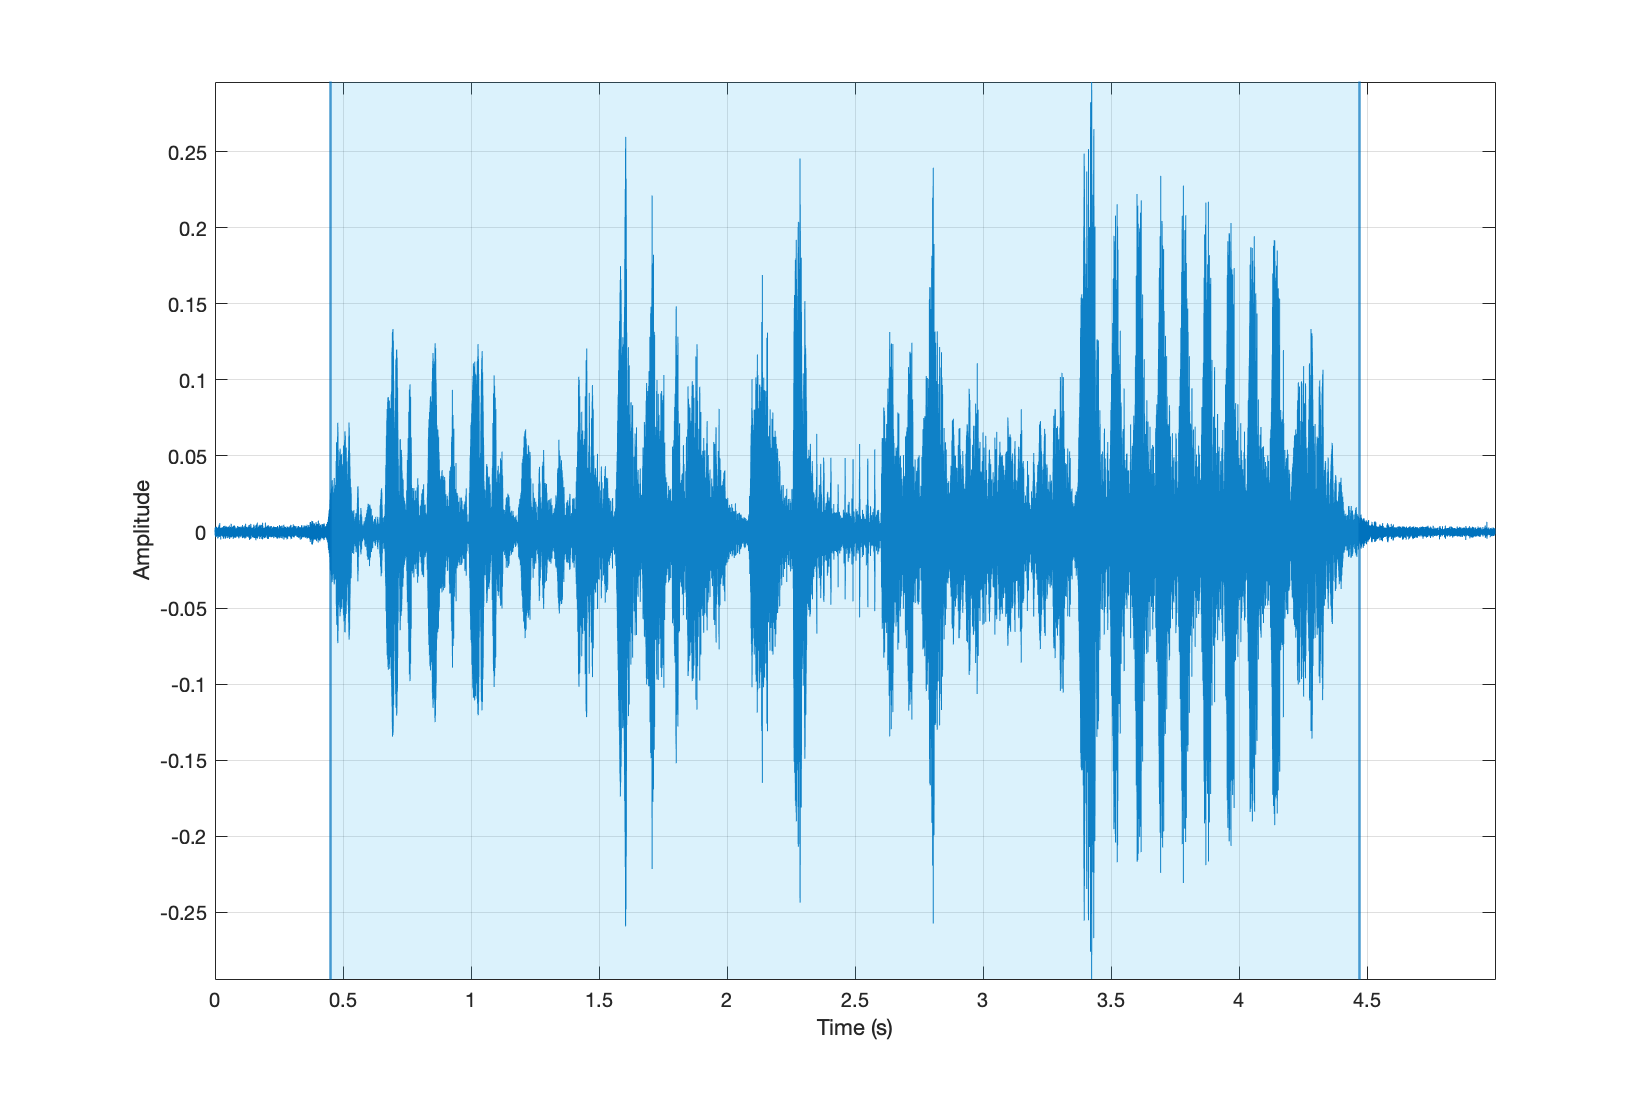
\includegraphics[width=\textwidth]{figures/detected_speech.png}
  \caption{Output of the \textit{detectSpeech} function for a recording of
  birdsong from a Eurasian wren. The highlighted section shows where the
algorithm has detected `speech', or in this case,
birdsong.}\label{fig:detected_speech}
\end{figure}

A highpass filter is then applied to the recording with a passband frequency of
450Hz. This value was chosen as most birdsong sits in the range of 1KHz ---
10Khz, and so lower frequencies can be attributed to background noise and
therefore their removal should reduce noise in the system without losing
important information. The reason why frequencies above 10Khz are not removed
is that, as can be seen from figure~\ref{fig:wren_call_song_spectrogram}, birds
typically produce higher frequency harmonics when vocalizing, shown as vertical
bands moving upwards from where syllables are located on the spectrogram. These
harmonics may capture useful information for the learning algorithm to utilise
and should therefore not be filtered out.

After these pre-processing steps have been taken, the audio is ready for
syllable segmentation.

\section{Segmentation}\label{sec:segmentation}

Recordings downloaded from XC were also chosen based on their length. Recordings
of duration 40 seconds to 120 seconds were preferred since they were likely to
be long enough to include enough variety of vocalizations from one individual
bird, but not too long so as to take up too much space on disk. In this thesis
it was preferred to have fewer samples from more individual as opposed to more
samples from fewer individuals for each species. The intention of this was to
introduce more variation in the training samples for each class, especially when
considering that many birds of the same species but residing in different
locations have demonstrated subtle variations in vocalizations, known as
dialects~\cite{baker1985biology}. As a general rule of thumb, a target of
roughly 50 training samples per individual was aimed for in this thesis.

This leads to the question of how to generate samples. In the literature there
seem to be two main ways of segmenting recordings into samples to be used for
training. The first is segmenting a recording into overlapping segments of a
certain length, typically in the range of 4 --- 11 seconds
(\cite{yan2021birdsong},~\cite{crous2019polyphonic}). This has the advantage
that all samples will be of fixed length and that the segmentation algorithm is
very simple. However, it will likely mean that some samples will contain only
background noise which, if used for training, will introduce noise into the
system. These noise samples therefore may need to be removed, either
manually~\cite{yan2021birdsong} or using an
algorithm~\cite{narasimhan2017simultaneous}. The other method involves
segmenting the recording into syllables
(\cite{fagerlund2007bird},~\cite{ramashini2022robust}). This has the advantage
that all training samples are likely to contain little or no noise. However the
samples will be of variable length, so steps will be needed to be taken in order
to compare the samples, such as adding padding or more advanced techniques like
dynamic time warping~\cite{somervuo2006parametric}. Syllable segmentation also
has the enticing prospect of being able to identify a bird species from a very
short sample. This could be useful in situations where a recording is mostly
corrupted by background noise but has a few small segments of clear birdsong.

In this work we attempt to combine the benefits of both approaches by first
segmenting a recording to retrieve the syllables using a process described in
Section~\ref{ssec:syllable_seg}. Then, for each syllable, the
following syllables are appended until a fixed sample length is reached. If a
syllable is added which pushes the sample length over the limit, then the sample
is trimmed at the fixed length. This approach is motivated by Somervuo et al.'s
work~\cite{somervuo2006parametric} in showing that training and classifying
using single syllables returns suboptimal results, whereas using sequences of
syllables gives much improved accuracy. Of course there is a tradeoff here
between training with longer sequences, and hence more information, versus
increased computational demand to perform training.

\begin{figure}[ht]
  \centering
  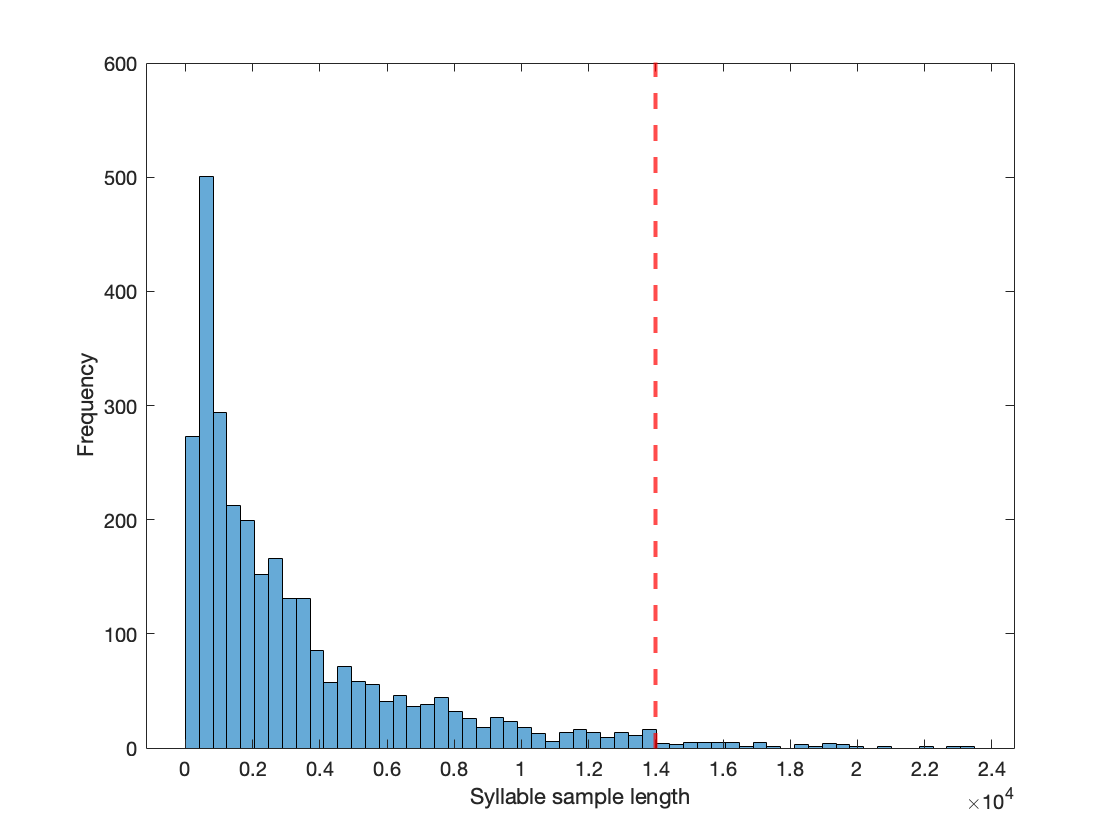
\includegraphics[width=\textwidth]{figures/syllable_sample_length.png}
  \caption{Histogram showing the frequency of different sample lengths for all
  training syllables. A candidate fixed sequence length is denoted by the red
dashed line.}\label{fig:syllable_sample_lengths}
\end{figure}

From figure~\ref{fig:syllable_sample_lengths}, we can see most syllable lengths
fall in the region $\left[ 200, 1236 \right]$ (the segmentation algorithm sets a
minimum of 200 samples for candidate syllables). Therefore a sequence of fixed
length about 14000 (denoted by the red dashed line) should contain between 10
and 70 syllables. The fixed length, equating to about 3ms duration, also ensures
that most sequences contain at least one full syllable. This approach ensures
the influence of background noise is kept to a minimum, while still maintaining
information related to the temporal evolution of a particular birdsong.

\subsection{Energy based syllable segmentation}\label{ssec:syllable_seg}

This algorithm was first proposed by Fagerlund~\cite{fagerlund2004automatic}
and has been used in various research papers since
(\cite{somervuo2006parametric},~\cite{ramashini2022robust}). Note that Fagerlund
proposed two different segmentation methods in the paper. In this thesis we use
the energy based segmentation method as it's relatively
simple to implement and its performance can be superior to the other method
proposed. The algorithm is computed in the following 3 phases:

\begin{enumerate}

  \item Determine the onsets and offsets of syllable candidates. Special
    attention has to be paid to the border effect~\cite{li2001classification},
    whereby the energy envelope near onsets and offsets fluctuates around a
    threshold.

  \item Syllable candidates that are within a certain temporal distance with
    each other are merged into one. The initial separation of candidates can
    likely be attributed to the border effect, and so the candidates can be
    thought of as originating from one syllable in reality.

  \item Syllable candidates that are shorter than a minimum threshold are
    removed. These candidates are often caused by random fluctuations in the
    signal energy and are unrelated to bird vocalizations.

\end{enumerate}

\subsubsection{Onset/offset detection}

The first phase considers the energy of an input signal. The energy envelope is
the key variable to use in determining the onset and offset of a syllable. The
general idea is that when the energy increases past a threshold, this marks the
start of a syllable candidate and when the energy then falls below the same
threshold, this marks the end of a syllable candidate. To calculate the energy
envelope, the recording is divided into overlapping frames.
Fagerlund~\cite{fagerlund2004automatic} recommends a frame size of 128 samples
and an overlap of 50\%. This corresponds to a frame length of roughly 3ms. Since
distance between syllables can be as short as 20ms, the frame size needs to be
small enough so that there are at least a few frames between candidates to be
able to efficiently discriminate between syllables.

Frames are first windowed using a Hanning window. The energy $E_i$ in the
decibel scale for frame $i$ is calculated as
\begin{equation}
  E_i = 10 \log_{10} \sum_{j=1}^{K} x{(i)}_{j}^2
\end{equation}
where $x{(i)}_j$ is the $j^{\text{th}}$ input signal sample value in the
$i^{\text{th}}$ frame and $K$ is the total number of samples in each frame, in
this case 128. The maximum energy of the entire signal is normalized to 0dB. The
initial noise level estimate is set to be equal to global minimum value of the
energy envelope and the threshold for the onset and offset detection is set to
half the noise estimate. The flow diagram for onset and offset detection can be
seen in figure <figure of flow chart>. In essence, the algorithm moves through
each frame and computes whether the frame should be assigned to a syllable or
not, updating noise and energy thresholds as it goes. The noise estimate is
updated as the average energy of frames already processed by the algorithm that
are not assigned to a syllable.

\subsubsection{Merging syllable candidates}

The algorithm may produce syllable candidates that are very temporally close
together. This may be from the bird producing short bursts of pulses that
constitute the same syllable, or it may be from the border effect. In both cases
the candidates can be considered as belonging to the same syllable and so can be
safely merged together. Candidates that are less than 15ms apart are selected
for merging~\cite{fagerlund2004automatic}.

<figures of segmentation>

Each segmented syllable is then stored as an individual \textit{wav} file in the
same directory as the original recording with a filename in the format
\textit{\{XCID\}\_i.wav} where \textit{XCID} is the XC id of the recording and
\textit{i} is the index of the syllable.

\section{Feature extraction}

Once syllables have been extracted and stored as individual audio files, they
are ready to be retrieved and converted to features. As mentioned in
Section~\ref{sec:segmentation}, before feature extraction is performed,
syllables are concatenated together until a minimum length is achieved.

\subsection{Cepstral coefficients}

The cepstral coefficients on which this thesis focuses are the MFCC and GTCC\@.
Both features are extracted using builtin \textit{MATLAB} functions
\textit{mfcc} and \textit{gtcc} respectively. The functions accept arguments
which affect how the routine processes input signals. To the best of the
author's knowledge, these arguments have not been explored in the field of
birdsong classification problems.

\subsubsection{MFCC}\label{sssec:mfcc}

A potentially overlooked parameter of MFCC extraction with regards to birdsong
classification using \textit{MATLAB} is the \textit{BandEdges} argument. This
argument provides the basis of the half-overlapped triangular filters that
\textit{mfcc} uses. By default, \textit{BandEdges} is a 42-element vector that
results in a 40-band filter bank constructed using 13 linearly-spaced filters,
with 133.3Hz separating their center frequencies, and 27 log-spaced filters,
separated by a factor of 1.0711703 in frequency~\cite{slaney1998auditory}. This
equates to a frequency range that spans approximately 133Hz to 6864Hz. This
range is well suited to human speech, of which MFCC is often used as a feature,
but may be less suitable for birdsong which can sometimes sit outside the normal
frequency range of human speech.

In this work we consider alternative constructions of the MFCC filter banks,
such as extending the range and adding more filters and assess the performance
of classifiers using the alternative MFCC filter banks in comparison with the
default.

\subsubsection{GTCC}

Like MFCC, GTCC has a potentially overlooked argument in
\textit{FrequencyRange}. This two-element row vector specifies the minimum and
maximum values in Hz of the gammatone filter bank used by the \textit{gtcc}
routine. The default value is \texttt{[50, fs/2]}, which could potentially be
fine-tuned for birdsong related problems since birdsong frequencies do not
typically go below 1Khz.

In this work we consider alternative values for the maximum and minimum
frequency of the gammatone filter bank and compare performance of classifiers
trained using the alternative GTCC representations with the default.

\subsection{MRCG}

\textit{MATLAB} provides no builtin functions for computing an MRCG, or even a
cochleagram, upon which the MRCG is based. To that end, custom code was
developed based on the toolbox developed by Kim and Hahn~\cite{kim2018voice}
which implements MRCG\@. The MRCG routine implemented in~\cite{kim2018voice}
uses a gammatone filter bank with a frequency range of \texttt{[50, 8000]},
which may not be suitable for birdsong problems. The work done in customising
the toolbox for this thesis extends the implementation to work with alternative
frequency ranges for the gammatone filter bank.

It's recommended to include the $\Delta$ and $\Delta\Delta$ values along with
the MRCG feature~\cite{chen2014feature}, so hereafter the term MRCG shall refer to
the base MRCG along with its $\Delta$ and $\Delta\Delta$ values. The same
applies to MFCC and GTCC\@.

Due to the high dimensionality of the MRCG feature and considering the
computational limitations of the machine upon which the training for this thesis
was performed, the MRCG feature would be best suited to a classifier which is
optimised for working with image data, such as CNNs\@. To that end, it won't
be used with SVMs in this work.

\section{Training}\label{sec:training}

To create the training cell array, syllables are retrieved and concatenated to form
a training sample, hereafter referred to as a sequence. A maximum limit of 40
sequences per individual is imposed to ensure enough variation while keeping
training times to a minimum. The number of training sequences used for both
classes can be seen in table~\ref{table:training_samples}.

\begin{table}[h!t]
\begin{center}
\begin{tabular}{c c c}
\toprule
Class & Individuals & Sequences \\ [0.5ex]
\midrule
Common blackbird (\textit{TURMER}) & 28 & 1107 \\
Common nightingale (\textit{LUSMEG}) & 28 & 1200 \\
\bottomrule
\end{tabular}
\caption{Number of training sequences for used for both
classes.}\label{table:training_samples}
\end{center}
\end{table}

The training cell is formed by vertically concatenating the two cell arrays
containing the training sequences to form a $2311 \times 1$ cell array. The
training labels are contained in a $2311 \times 1$ categorical array with a
\textit{TURMER} category labelling a blackbird sequence and \textit{LUSMEG}
labelling a nightingale sequence.

All training is performed on an Apple MacBook Pro (late 2013) running OSX
11.5.2.

\subsection{SVMs}

All SVM models are implemented using \textit{MATLAB's} \texttt{fitcsvm}
function provided in the Statistics and Machine Learning Toolbox.

SVMs require each training sample to be a row vector. To convert the training
cell array to the required matrix format, a function can be applied to each cell
using the \texttt{cellfun} function to extract the desired feature and flatten
the output to a row vector. A simple routine can then be applied to convert the
cell array to a matrix of numerical data, the required format for
\texttt{fitcsvm}. The training labels cell array mentioned in the previous
section requires no transformation.

\subsubsection{Linear}

Linear SVMs are trained by supplying a \textit{KernelFunction} argument set to
\textit{linear} to the \texttt{fitcsvm} function. Linear SVMs are reasonably
simple to fit as they have fewer parameters than SVMs utilising other kernel
functions. The key parameter to tune for here is the \textit{BoxConstraint},
which controls the trade-off between maximizing the margin between classes and
minimizing the classification error. This is the constant $C$ in Equation
(\ref{eq:svm_nonlinear_mapping_slack}). The \textit{Standardize} parameter
controls whether data is standardized before fitting, and can also affect the
performance of the model. In this work, KFold cross-validation (KF) was selected
to optimize the parameters, with $K=7$ folds. This is motivated by other
research taking the same approach with promising
results~\cite{ramashini2022robust}.

Figure~\ref{fig:linear_optim} shows where the optimum values of
\textit{BoxConstraint} and \textit{Standardize} lie for a linear SVM\@. As can
be seen, the \textit{Standardize} parameter makes a slight difference on model
performance, whereas \textit{BoxConstraint} makes a significant difference, with
lower values preferred. A lower value means that the model has greater
flexibility in misclassifying training samples for the benefit of better
generalization.

\begin{figure}[ht]
  \centering
  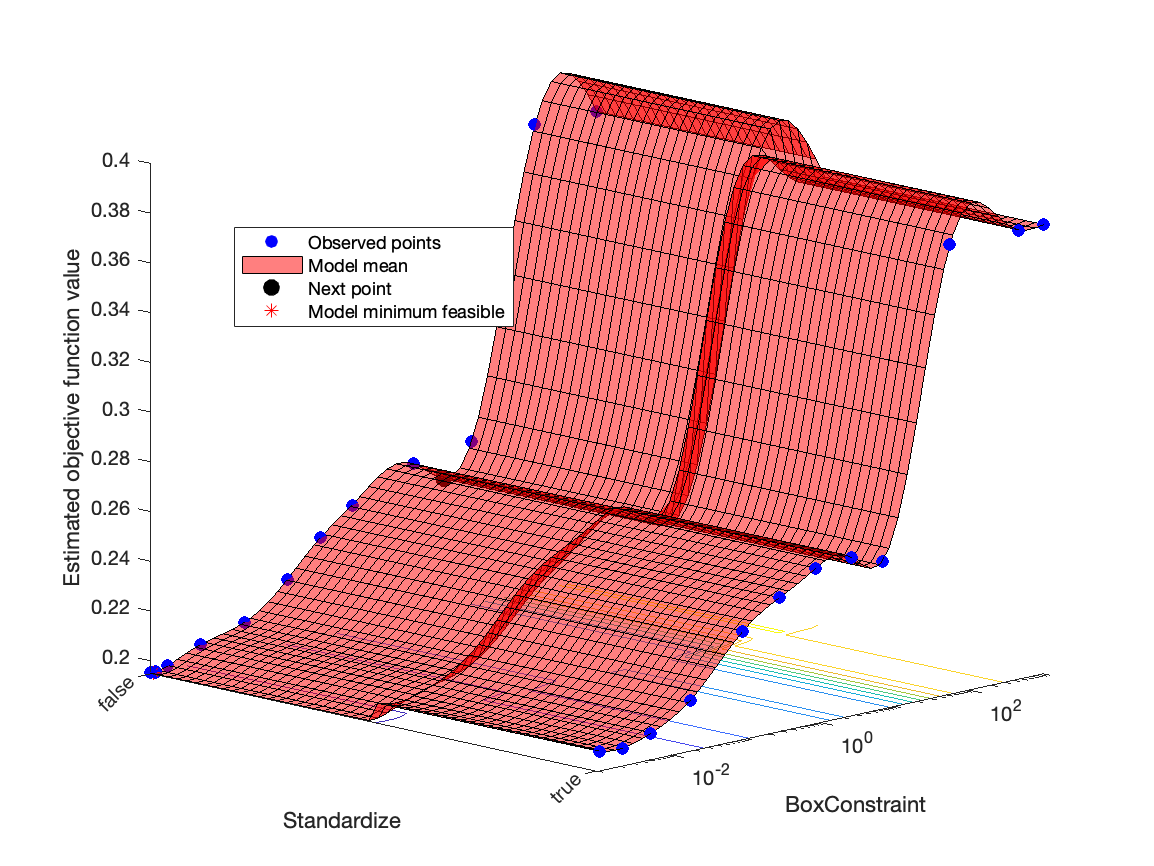
\includegraphics[width=\textwidth]{figures/linear_optim.png}
  \caption{Plot showing optimum values of the \textit{BoxConstraint} and
  \textit{Standardize} parameters when fitting a linear SVM.\ The optimum values
are located where the objective function is at a
minimum.}\label{fig:linear_optim}
\end{figure}

\subsubsection{RBF}

RBF SVMs are able to fit more complex decision boundaries by projecting data
into a higher dimensional space, which is controlled by the hyperparameter
\textit{KernelScale}. RBF SVMs are also sensitive to the \textit{BoxConstraint}
parameter. 7-fold cross validation was performed using a \texttt{cvpartition}
and supplying a \textit{OptimizeHyperparameters} argument set to \textit{auto}
to \texttt{fitcsvm}. A value of \textit{auto} means that both
\textit{KernelScale} and \textit{BoxConstraint} are optimised during training.

Figure~\ref{fig:rbf_optim} shows where the optimum values of
\textit{BoxConstraint} and \textit{KernelScale} lie for a RBF SVM\@. Both
parameters are shown to have an impact on the model performance, with high
values of \textit{BoxConstraint} and mid-range values of \textit{KernelScale}
preferred. <what does kernel scale do?>

\begin{figure}[ht]
  \centering
  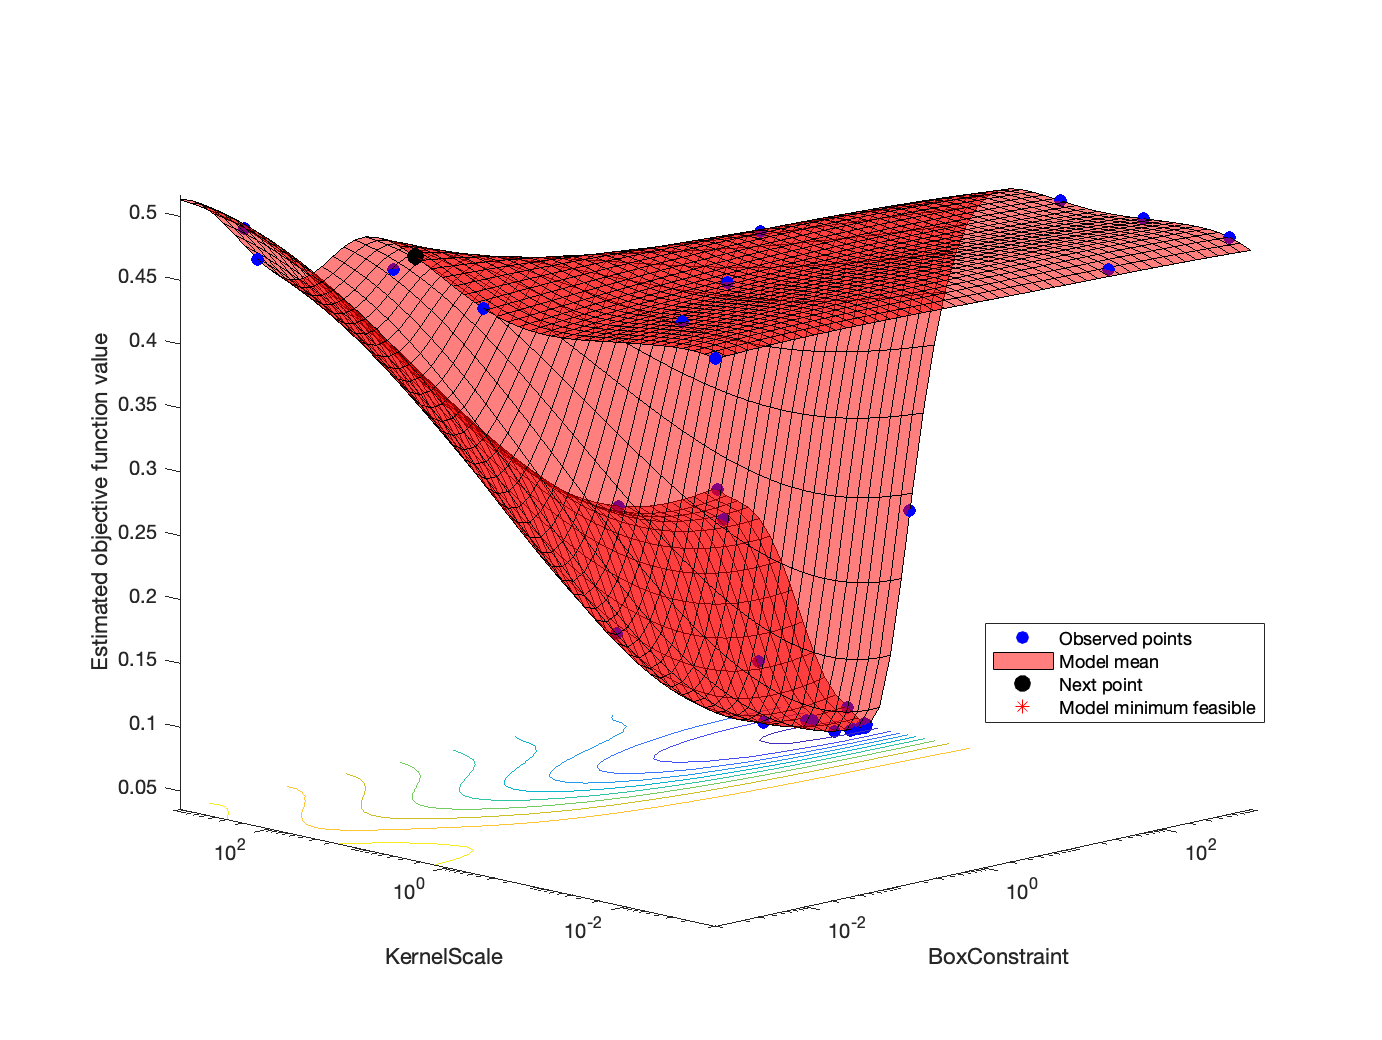
\includegraphics[width=\textwidth]{figures/rbf_optim.png}
  \caption{Plot showing optimum values of the \textit{BoxConstraint} and
  \textit{KernelScale} parameters when fitting a RBF SVM.\ The optimum values
are located where the objective function is at a
minimum.}\label{fig:rbf_optim}
\end{figure}

\subsection{Neural networks}

\section{Evaluation}

After the recordings from each class reserved for testing have undergone
pre-processing and segmentation, the segmented syllables undergo the same
routine described in Section~\ref{sec:training} to generate the testing
sequences. The number of testing sequences used for both classes can be seen in
table~\ref{table:testing_samples}.

\begin{table}[h!t]
\begin{center}
\begin{tabular}{c c c}
\toprule
Class & Individuals & Sequences \\ [0.5ex]
\midrule
Common blackbird (\textit{TURMER}) & 9 & 360 \\
Common nightingale (\textit{LUSMEG}) & 10 & 400 \\
\bottomrule
\end{tabular}
\caption{Number of testing sequences for used for both
classes.}\label{table:testing_samples}
\end{center}
\end{table}

A testing cell is created in the same way as the training cell and is used for
evaluating all models in this thesis.

\subsection{AUC}

As mentioned in Section~\ref{sec:eval_metrics}, the AUC metric is commonly used
for binary classification problems, and has been frequently used as a metric in
birdsong classification problems. Further to the advantages listed in 
previously, the AUC benefits from being unaffected from class imbalances.
Although the positive and negative classes are only slightly imbalanced in this
work (see Table~\ref{table:training_samples}), it makes sense to use a metric
that is unaffected by class imbalance all the same.

The AUC is calculated using the \texttt{perfcurve} function which checks the
class prediction scores returned by the model against the true labels.

\subsection{Classification accuracy}

Since the classes are only slightly imbalanced, the classification accuracy
provides a reasonably unbiased, quick, and easily interpretable snapshot at how
well a model has performed. It is calculated as
\begin{equation}
A = \frac{1}{N}\sum_{i=1}^{N} \mathbb{I}[\bar{y}_i = y_i]
\end{equation}
where $N$ is the number of test samples, $\bar{y}$ is a predicted label, $y$
is the groundtruth label, and $\mathbb{I}$ is the indicator function.

\section{Extensions of methodology}
